% ===================== Phase 1: Architectural model =====================
% Paste into the group's IEEE conference template (% ===================== Phase 1: Architectural model =====================
% Paste into the group's IEEE conference template (% ===================== Phase 1: Architectural model =====================
% Paste into the group's IEEE conference template (% ===================== Phase 1: Architectural model =====================
% Paste into the group's IEEE conference template (\input{phase1}). Needs graphicx.
% Tables and figures do not count toward the 3-page text limit, so the requirements
% and stakeholders live in Table I and the prose stays short.
\section{Phase 1: Architectural Model}\label{sec:phase1}

\subsection{Requirements and Stakeholders}
Table~\ref{tab:requirements} lists the requirements and stakeholders. The NFRs
are measurable, so later phases can test them: NFR1 in Phases~2--3, NFR2 in Phase~4.

% NFR targets are set from the stakeholders' needs, not from measurements. If you
% change them, keep them measurable. NFR2's 5 s must match the health-check period
% chosen in Phase 4.
\begin{table}[t]
\caption{Requirements and stakeholders}
\label{tab:requirements}
\centering
\footnotesize
\begin{tabular}{@{}p{0.19\columnwidth}p{0.75\columnwidth}@{}}
\hline
\textbf{ID} & \textbf{Requirement} \\
\hline
FR1 & \emph{Keyword count.} Given a text ID and a keyword, return the exact
number of whole-word occurrences of the keyword in that text. A word is a maximal
run of letters or digits, optionally joined by apostrophes, compared after Unicode
case folding; all other characters separate words. A request for an unknown text,
or with a keyword that is not exactly one word, is rejected with an error instead
of being answered with 0. \\
FR2 & \emph{Hot keywords.} Count every valid request per keyword and, on request,
return the $k$ most requested keywords with their request counts, over all
clients and texts. \\
NFR1 & \emph{Latency.} Measured at the client, mean latency $\le 10$\,ms and
99th-percentile latency $\le 50$\,ms at the offered load. Repeated requests are
answered from an in-memory cache. When one server cannot meet this, capacity is
added by replicating the server, without changes to clients. \\
NFR2 & \emph{Availability.} When one server replica crashes the service keeps
answering: the failed replica receives no new requests within 5\,s of failing,
and receives requests again within 5\,s of recovering. \\
\hline
\textbf{Stakeholder} & \textbf{Role} \\
\hline
\raggedright Client developer & Builds applications on the service, e.g., text analytics or
plagiarism detection, and calls it through its RPC interface. Needs correct counts
(FR1), a stable interface and predictable latency (NFR1); determines the request
mix and rate. \\
Operator & Deploys and configures the containers (corpus, cache size, number of
replicas), monitors latency and replica health, and restores failed servers.
Needs NFR1 to hold as load grows, and NFR2; uses FR2 to understand demand. \\
\hline
\end{tabular}
\end{table}

\subsection{Architecture}
Fig.~\ref{fig:arch} shows the architecture, in the client--server style: clients
issue requests; the server answers them and keeps no per-client state, so any
replica can serve any request (needed in Phase~3). The containers form three tiers,
a layered organization of the client--server system: client, application server,
and data (Redis and the corpus).

\emph{Components.} Clients call the service through a client stub
(\texttt{WordCountClient}), used by both the command-line tool and the load
generator. The server runs an RPyC \texttt{ThreadedServer} (a thread per
connection) hosting \texttt{WordCountService}, which validates a request, consults
the cache and, on a miss, counts. \texttt{TextCatalog} holds the texts, read once
at startup from a read-only volume and tokenized; clients refer to a text by its
ID (the file name), never by a path. \texttt{CountCache} encapsulates Redis, which
stores one count per text and word (no expiry, as texts never change; LRU eviction
bounds memory) and a sorted set of request counts per keyword (FR2).

\emph{Connectors.} (1)~Client--server: RPyC over TCP, synchronous request--reply,
one connection per request. Replies are plain tuples, which RPyC copies by value;
a list or object would arrive as a remote reference whose every use is another
round trip to that particular server. (2)~Server--Redis: RESP over TCP; lookup and
hot-keyword update share one pipelined round trip, and a miss adds a \texttt{SET}.
(3)~Server--corpus: a file read at startup.

\begin{figure}[t]
\centering
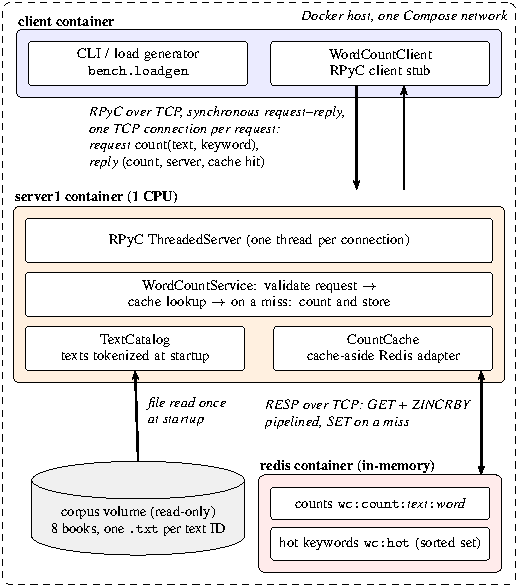
\includegraphics[width=\columnwidth]{figures/architecture_phase2}
\caption{Client--server architecture of the word count service (Phases 1--2).
Boxes are containers on one Docker host; arrows are connectors.}
\label{fig:arch}
\end{figure}

\subsection{Alternative Architectural Styles}
\emph{Peer-to-peer.} Each peer would store some texts and cache its own results.
A structured overlay such as a Chord distributed hash table~\cite{stoica2001chord}
maps a text ID to the responsible peer in $O(\log N)$ hops, and successor peers
keep replicas. This removes the server as bottleneck and single point of failure,
and capacity grows with the peers. Here the costs dominate: every lookup adds
overlay hops where client--server needs one; FR2 needs a global ranking, but
request statistics would be spread over all peers; churn forces re-replication;
and peers from other domains of authority could return wrong counts that clients
cannot check. For a small, centrally administered corpus, P2P is feasible but
unsuitable.

\emph{Publish--subscribe.} Clients would publish requests to a topic; servers
take them as competing consumers and publish answers on per-client reply topics,
matched by correlation IDs. The broker decouples both sides in time and
space~\cite{eugster2003pubsub}: servers can be added unnoticed and bursts are
buffered. But a count is a synchronous query: the client waits anyway, so the
decoupling buys little, while the broker adds a hop and queueing to every request
(against NFR1) and is one more component that can become a bottleneck or single
point of failure. Publish--subscribe does fit pushing hot-keyword updates (FR2) to
subscribers such as dashboards; counting stays request--reply client--server.
). Needs graphicx.
% Tables and figures do not count toward the 3-page text limit, so the requirements
% and stakeholders live in Table I and the prose stays short.
\section{Phase 1: Architectural Model}\label{sec:phase1}

\subsection{Requirements and Stakeholders}
Table~\ref{tab:requirements} lists the requirements and stakeholders. The NFRs
are measurable, so later phases can test them: NFR1 in Phases~2--3, NFR2 in Phase~4.

% NFR targets are set from the stakeholders' needs, not from measurements. If you
% change them, keep them measurable. NFR2's 5 s must match the health-check period
% chosen in Phase 4.
\begin{table}[t]
\caption{Requirements and stakeholders}
\label{tab:requirements}
\centering
\footnotesize
\begin{tabular}{@{}p{0.19\columnwidth}p{0.75\columnwidth}@{}}
\hline
\textbf{ID} & \textbf{Requirement} \\
\hline
FR1 & \emph{Keyword count.} Given a text ID and a keyword, return the exact
number of whole-word occurrences of the keyword in that text. A word is a maximal
run of letters or digits, optionally joined by apostrophes, compared after Unicode
case folding; all other characters separate words. A request for an unknown text,
or with a keyword that is not exactly one word, is rejected with an error instead
of being answered with 0. \\
FR2 & \emph{Hot keywords.} Count every valid request per keyword and, on request,
return the $k$ most requested keywords with their request counts, over all
clients and texts. \\
NFR1 & \emph{Latency.} Measured at the client, mean latency $\le 10$\,ms and
99th-percentile latency $\le 50$\,ms at the offered load. Repeated requests are
answered from an in-memory cache. When one server cannot meet this, capacity is
added by replicating the server, without changes to clients. \\
NFR2 & \emph{Availability.} When one server replica crashes the service keeps
answering: the failed replica receives no new requests within 5\,s of failing,
and receives requests again within 5\,s of recovering. \\
\hline
\textbf{Stakeholder} & \textbf{Role} \\
\hline
\raggedright Client developer & Builds applications on the service, e.g., text analytics or
plagiarism detection, and calls it through its RPC interface. Needs correct counts
(FR1), a stable interface and predictable latency (NFR1); determines the request
mix and rate. \\
Operator & Deploys and configures the containers (corpus, cache size, number of
replicas), monitors latency and replica health, and restores failed servers.
Needs NFR1 to hold as load grows, and NFR2; uses FR2 to understand demand. \\
\hline
\end{tabular}
\end{table}

\subsection{Architecture}
Fig.~\ref{fig:arch} shows the architecture, in the client--server style: clients
issue requests; the server answers them and keeps no per-client state, so any
replica can serve any request (needed in Phase~3). The containers form three tiers,
a layered organization of the client--server system: client, application server,
and data (Redis and the corpus).

\emph{Components.} Clients call the service through a client stub
(\texttt{WordCountClient}), used by both the command-line tool and the load
generator. The server runs an RPyC \texttt{ThreadedServer} (a thread per
connection) hosting \texttt{WordCountService}, which validates a request, consults
the cache and, on a miss, counts. \texttt{TextCatalog} holds the texts, read once
at startup from a read-only volume and tokenized; clients refer to a text by its
ID (the file name), never by a path. \texttt{CountCache} encapsulates Redis, which
stores one count per text and word (no expiry, as texts never change; LRU eviction
bounds memory) and a sorted set of request counts per keyword (FR2).

\emph{Connectors.} (1)~Client--server: RPyC over TCP, synchronous request--reply,
one connection per request. Replies are plain tuples, which RPyC copies by value;
a list or object would arrive as a remote reference whose every use is another
round trip to that particular server. (2)~Server--Redis: RESP over TCP; lookup and
hot-keyword update share one pipelined round trip, and a miss adds a \texttt{SET}.
(3)~Server--corpus: a file read at startup.

\begin{figure}[t]
\centering
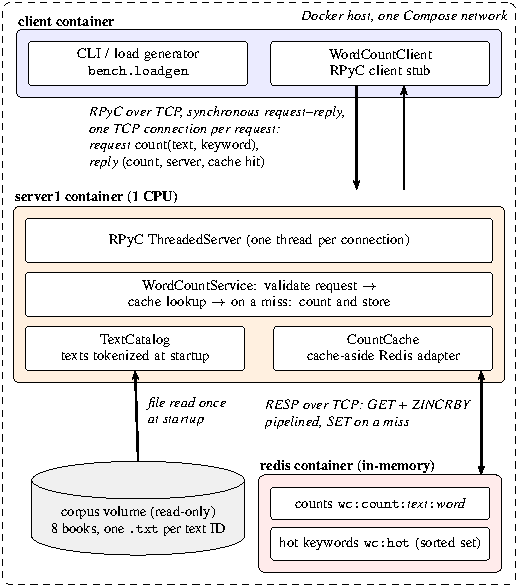
\includegraphics[width=\columnwidth]{figures/architecture_phase2}
\caption{Client--server architecture of the word count service (Phases 1--2).
Boxes are containers on one Docker host; arrows are connectors.}
\label{fig:arch}
\end{figure}

\subsection{Alternative Architectural Styles}
\emph{Peer-to-peer.} Each peer would store some texts and cache its own results.
A structured overlay such as a Chord distributed hash table~\cite{stoica2001chord}
maps a text ID to the responsible peer in $O(\log N)$ hops, and successor peers
keep replicas. This removes the server as bottleneck and single point of failure,
and capacity grows with the peers. Here the costs dominate: every lookup adds
overlay hops where client--server needs one; FR2 needs a global ranking, but
request statistics would be spread over all peers; churn forces re-replication;
and peers from other domains of authority could return wrong counts that clients
cannot check. For a small, centrally administered corpus, P2P is feasible but
unsuitable.

\emph{Publish--subscribe.} Clients would publish requests to a topic; servers
take them as competing consumers and publish answers on per-client reply topics,
matched by correlation IDs. The broker decouples both sides in time and
space~\cite{eugster2003pubsub}: servers can be added unnoticed and bursts are
buffered. But a count is a synchronous query: the client waits anyway, so the
decoupling buys little, while the broker adds a hop and queueing to every request
(against NFR1) and is one more component that can become a bottleneck or single
point of failure. Publish--subscribe does fit pushing hot-keyword updates (FR2) to
subscribers such as dashboards; counting stays request--reply client--server.
). Needs graphicx.
% Tables and figures do not count toward the 3-page text limit, so the requirements
% and stakeholders live in Table I and the prose stays short.
\section{Phase 1: Architectural Model}\label{sec:phase1}

\subsection{Requirements and Stakeholders}
Table~\ref{tab:requirements} lists the requirements and stakeholders. The NFRs
are measurable, so later phases can test them: NFR1 in Phases~2--3, NFR2 in Phase~4.

% NFR targets are set from the stakeholders' needs, not from measurements. If you
% change them, keep them measurable. NFR2's 5 s must match the health-check period
% chosen in Phase 4.
\begin{table}[t]
\caption{Requirements and stakeholders}
\label{tab:requirements}
\centering
\footnotesize
\begin{tabular}{@{}p{0.19\columnwidth}p{0.75\columnwidth}@{}}
\hline
\textbf{ID} & \textbf{Requirement} \\
\hline
FR1 & \emph{Keyword count.} Given a text ID and a keyword, return the exact
number of whole-word occurrences of the keyword in that text. A word is a maximal
run of letters or digits, optionally joined by apostrophes, compared after Unicode
case folding; all other characters separate words. A request for an unknown text,
or with a keyword that is not exactly one word, is rejected with an error instead
of being answered with 0. \\
FR2 & \emph{Hot keywords.} Count every valid request per keyword and, on request,
return the $k$ most requested keywords with their request counts, over all
clients and texts. \\
NFR1 & \emph{Latency.} Measured at the client, mean latency $\le 10$\,ms and
99th-percentile latency $\le 50$\,ms at the offered load. Repeated requests are
answered from an in-memory cache. When one server cannot meet this, capacity is
added by replicating the server, without changes to clients. \\
NFR2 & \emph{Availability.} When one server replica crashes the service keeps
answering: the failed replica receives no new requests within 5\,s of failing,
and receives requests again within 5\,s of recovering. \\
\hline
\textbf{Stakeholder} & \textbf{Role} \\
\hline
\raggedright Client developer & Builds applications on the service, e.g., text analytics or
plagiarism detection, and calls it through its RPC interface. Needs correct counts
(FR1), a stable interface and predictable latency (NFR1); determines the request
mix and rate. \\
Operator & Deploys and configures the containers (corpus, cache size, number of
replicas), monitors latency and replica health, and restores failed servers.
Needs NFR1 to hold as load grows, and NFR2; uses FR2 to understand demand. \\
\hline
\end{tabular}
\end{table}

\subsection{Architecture}
Fig.~\ref{fig:arch} shows the architecture, in the client--server style: clients
issue requests; the server answers them and keeps no per-client state, so any
replica can serve any request (needed in Phase~3). The containers form three tiers,
a layered organization of the client--server system: client, application server,
and data (Redis and the corpus).

\emph{Components.} Clients call the service through a client stub
(\texttt{WordCountClient}), used by both the command-line tool and the load
generator. The server runs an RPyC \texttt{ThreadedServer} (a thread per
connection) hosting \texttt{WordCountService}, which validates a request, consults
the cache and, on a miss, counts. \texttt{TextCatalog} holds the texts, read once
at startup from a read-only volume and tokenized; clients refer to a text by its
ID (the file name), never by a path. \texttt{CountCache} encapsulates Redis, which
stores one count per text and word (no expiry, as texts never change; LRU eviction
bounds memory) and a sorted set of request counts per keyword (FR2).

\emph{Connectors.} (1)~Client--server: RPyC over TCP, synchronous request--reply,
one connection per request. Replies are plain tuples, which RPyC copies by value;
a list or object would arrive as a remote reference whose every use is another
round trip to that particular server. (2)~Server--Redis: RESP over TCP; lookup and
hot-keyword update share one pipelined round trip, and a miss adds a \texttt{SET}.
(3)~Server--corpus: a file read at startup.

\begin{figure}[t]
\centering
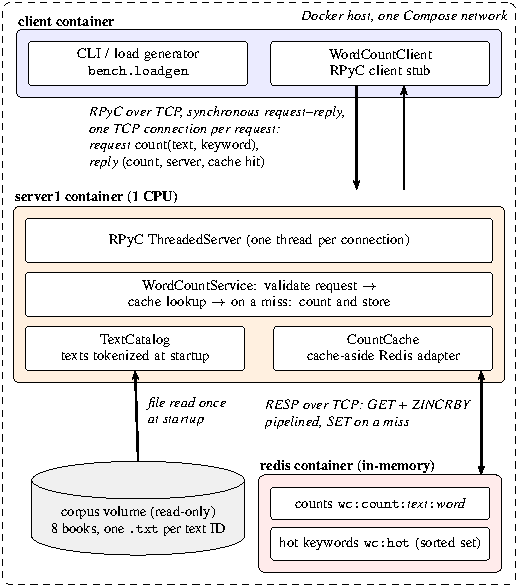
\includegraphics[width=\columnwidth]{figures/architecture_phase2}
\caption{Client--server architecture of the word count service (Phases 1--2).
Boxes are containers on one Docker host; arrows are connectors.}
\label{fig:arch}
\end{figure}

\subsection{Alternative Architectural Styles}
\emph{Peer-to-peer.} Each peer would store some texts and cache its own results.
A structured overlay such as a Chord distributed hash table~\cite{stoica2001chord}
maps a text ID to the responsible peer in $O(\log N)$ hops, and successor peers
keep replicas. This removes the server as bottleneck and single point of failure,
and capacity grows with the peers. Here the costs dominate: every lookup adds
overlay hops where client--server needs one; FR2 needs a global ranking, but
request statistics would be spread over all peers; churn forces re-replication;
and peers from other domains of authority could return wrong counts that clients
cannot check. For a small, centrally administered corpus, P2P is feasible but
unsuitable.

\emph{Publish--subscribe.} Clients would publish requests to a topic; servers
take them as competing consumers and publish answers on per-client reply topics,
matched by correlation IDs. The broker decouples both sides in time and
space~\cite{eugster2003pubsub}: servers can be added unnoticed and bursts are
buffered. But a count is a synchronous query: the client waits anyway, so the
decoupling buys little, while the broker adds a hop and queueing to every request
(against NFR1) and is one more component that can become a bottleneck or single
point of failure. Publish--subscribe does fit pushing hot-keyword updates (FR2) to
subscribers such as dashboards; counting stays request--reply client--server.
). Needs graphicx.
% Tables and figures do not count toward the 3-page text limit, so the requirements
% and stakeholders live in Table I and the prose stays short.
\section{Phase 1: Architectural Model}\label{sec:phase1}

\subsection{Requirements and Stakeholders}
Table~\ref{tab:requirements} lists the requirements and stakeholders. The NFRs
are measurable, so later phases can test them: NFR1 in Phases~2--3, NFR2 in Phase~4.

% NFR targets are set from the stakeholders' needs, not from measurements. If you
% change them, keep them measurable. NFR2's 5 s must match the health-check period
% chosen in Phase 4.
\begin{table}[t]
\caption{Requirements and stakeholders}
\label{tab:requirements}
\centering
\footnotesize
\begin{tabular}{@{}p{0.19\columnwidth}p{0.75\columnwidth}@{}}
\hline
\textbf{ID} & \textbf{Requirement} \\
\hline
FR1 & \emph{Keyword count.} Given a text ID and a keyword, return the exact
number of whole-word occurrences of the keyword in that text. A word is a maximal
run of letters or digits, optionally joined by apostrophes, compared after Unicode
case folding; all other characters separate words. A request for an unknown text,
or with a keyword that is not exactly one word, is rejected with an error instead
of being answered with 0. \\
FR2 & \emph{Hot keywords.} Count every valid request per keyword and, on request,
return the $k$ most requested keywords with their request counts, over all
clients and texts. \\
NFR1 & \emph{Latency.} Measured at the client, mean latency $\le 10$\,ms and
99th-percentile latency $\le 50$\,ms at the offered load. Repeated requests are
answered from an in-memory cache. When one server cannot meet this, capacity is
added by replicating the server, without changes to clients. \\
NFR2 & \emph{Availability.} When one server replica crashes the service keeps
answering: the failed replica receives no new requests within 5\,s of failing,
and receives requests again within 5\,s of recovering. \\
\hline
\textbf{Stakeholder} & \textbf{Role} \\
\hline
\raggedright Client developer & Builds applications on the service, e.g., text analytics or
plagiarism detection, and calls it through its RPC interface. Needs correct counts
(FR1), a stable interface and predictable latency (NFR1); determines the request
mix and rate. \\
Operator & Deploys and configures the containers (corpus, cache size, number of
replicas), monitors latency and replica health, and restores failed servers.
Needs NFR1 to hold as load grows, and NFR2; uses FR2 to understand demand. \\
\hline
\end{tabular}
\end{table}

\subsection{Architecture}
Fig.~\ref{fig:arch} shows the architecture, in the client--server style: clients
issue requests; the server answers them and keeps no per-client state, so any
replica can serve any request (needed in Phase~3). The containers form three tiers,
a layered organization of the client--server system: client, application server,
and data (Redis and the corpus).

\emph{Components.} Clients call the service through a client stub
(\texttt{WordCountClient}), used by both the command-line tool and the load
generator. The server runs an RPyC \texttt{ThreadedServer} (a thread per
connection) hosting \texttt{WordCountService}, which validates a request, consults
the cache and, on a miss, counts. \texttt{TextCatalog} holds the texts, read once
at startup from a read-only volume and tokenized; clients refer to a text by its
ID (the file name), never by a path. \texttt{CountCache} encapsulates Redis, which
stores one count per text and word (no expiry, as texts never change; LRU eviction
bounds memory) and a sorted set of request counts per keyword (FR2).

\emph{Connectors.} (1)~Client--server: RPyC over TCP, synchronous request--reply,
one connection per request. Replies are plain tuples, which RPyC copies by value;
a list or object would arrive as a remote reference whose every use is another
round trip to that particular server. (2)~Server--Redis: RESP over TCP; lookup and
hot-keyword update share one pipelined round trip, and a miss adds a \texttt{SET}.
(3)~Server--corpus: a file read at startup.

\begin{figure}[t]
\centering
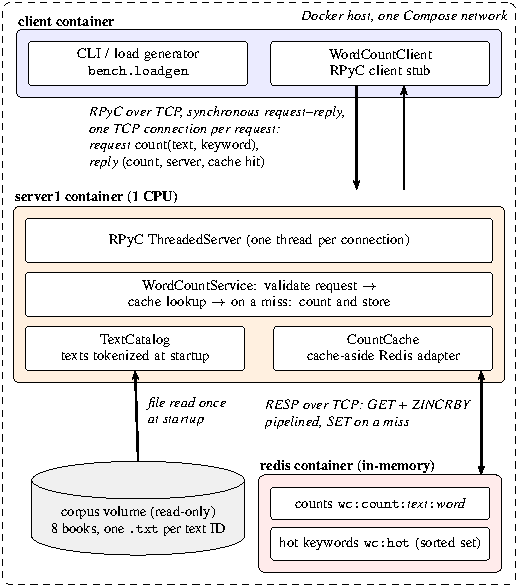
\includegraphics[width=\columnwidth]{figures/architecture_phase2}
\caption{Client--server architecture of the word count service (Phases 1--2).
Boxes are containers on one Docker host; arrows are connectors.}
\label{fig:arch}
\end{figure}

\subsection{Alternative Architectural Styles}
\emph{Peer-to-peer.} Each peer would store some texts and cache its own results.
A structured overlay such as a Chord distributed hash table~\cite{stoica2001chord}
maps a text ID to the responsible peer in $O(\log N)$ hops, and successor peers
keep replicas. This removes the server as bottleneck and single point of failure,
and capacity grows with the peers. Here the costs dominate: every lookup adds
overlay hops where client--server needs one; FR2 needs a global ranking, but
request statistics would be spread over all peers; churn forces re-replication;
and peers from other domains of authority could return wrong counts that clients
cannot check. For a small, centrally administered corpus, P2P is feasible but
unsuitable.

\emph{Publish--subscribe.} Clients would publish requests to a topic; servers
take them as competing consumers and publish answers on per-client reply topics,
matched by correlation IDs. The broker decouples both sides in time and
space~\cite{eugster2003pubsub}: servers can be added unnoticed and bursts are
buffered. But a count is a synchronous query: the client waits anyway, so the
decoupling buys little, while the broker adds a hop and queueing to every request
(against NFR1) and is one more component that can become a bottleneck or single
point of failure. Publish--subscribe does fit pushing hot-keyword updates (FR2) to
subscribers such as dashboards; counting stays request--reply client--server.
